% !TEX program = xelatex
\documentclass[twocolumn]{article}
\usepackage{ctex}
\usepackage{amsmath}
\usepackage{graphicx}
\usepackage{xcolor}
\usepackage{listings}
\usepackage{geometry}
\usepackage{fancyhdr}
\usepackage{tabularx}
\usepackage{booktabs}
\usepackage{hyperref}
\usepackage{forest}
\usepackage{float}


% --- 页面布局 ---
\geometry{a4paper, left=2cm, right=2cm, top=2.5cm, bottom=2.5cm, columnsep=1cm}

% --- 代码高亮配置 ---
\definecolor{codegreen}{rgb}{0,0.6,0}
\definecolor{codegray}{rgb}{0.5,0.5,0.5}
\definecolor{codepurple}{rgb}{0.58,0,0.82}
\definecolor{backcolour}{rgb}{0.95,0.95,0.92}

\lstdefinestyle{mystyle}{
    backgroundcolor=\color{backcolour},   
    commentstyle=\color{codegreen},
    keywordstyle=\color{magenta},
    numberstyle=\tiny\color{codegray},
    stringstyle=\color{codepurple},
    basicstyle=\ttfamily\footnotesize,
    breakatwhitespace=false,         
    breaklines=true,                 
    captionpos=b,                    
    keepspaces=true,                 
    numbers=left,                    
    numbersep=5pt,                  
    showspaces=false,                
    showstringspaces=false,
    showtabs=false,                  
    tabsize=2,
    columns=flexible,
    literate={\_}{{\textunderscore}}1,
    mathescape=false,
    texcl=false
}
\lstset{style=mystyle}

% --- 自定义 listings 语言 ---
\lstdefinelanguage{flex}{
    keywords={%
        options, case-insensitive, noyywrap, yylineno,
        x, s,
    },
    sensitive=false,
    morecomment=[l][\color{codegreen}]{//},
    morecomment=[s][\color{codegreen}]{/*}{*/},
    morecomment=[s][\color{codegreen}]{\%\{}{\%\}},
    morestring=[b][\color{codepurple}]",
    alsoletter={-,>},
    morekeywords=[2]{BEGIN, ECHO, REJECT, yylval, yytext, yyleng, yylex, curr_lineno},
    mathescape=false,
    texcl=false,
}

\lstdefinelanguage{cool}{
    keywords={%
        class, inherits, if, then, else, fi, while, loop, pool, let, in, case, of, esac, new, isvoid, not, true, false,
        Int, String, Bool, Object, SELF_TYPE, self
    },
    sensitive=false,
    morecomment=[l][\color{codegreen}]{--},
    morecomment=[s][\color{codegreen}]{(*}{*)},
    morestring=[b][\color{codepurple}]",
    morekeywords=[2]{},
}


% --- 页眉页脚 ---
\pagestyle{fancy}
\fancyhf{}
\fancyhead[L]{COOL 词法分析器实验报告}
\fancyhead[R]{\thepage}
\fancyfoot[C]{\small \copyright\ 2025}
\renewcommand{\headrulewidth}{0.4pt}
\renewcommand{\footrulewidth}{0.4pt}

% --- 标题 ---
\title{
    \vspace{-1cm} % 调整标题位置
    \textbf{COOL 语言词法分析器开发报告} \\
    \large \texttt{Compiler Principle Assignment}
}
\author{
    姓名: \textcolor{red}{谭润} \\
    学号: \textcolor{red}{20238131027} \\
    班级: \textcolor{red}{大数据二班} \\
    项目代码:\href{https://github.com/tanrun0/school_homework_code/tree/main/compiler/shiyan2}{Github链接}
}
\date{\today}

% --- 文档开始 ---
\begin{document}

\maketitle
\thispagestyle{fancy} % 首页也使用fancy样式

\begin{abstract}
\noindent
本实验基于 Flex 工具实现了 COOL语言词法分析器的设计与开发过程。首先深入阐释了 Flex 的核心原理,包括通过正则表达式构建 NFA、经子集构造法转化为 DFA 并最小化的自动机生成流程,以及最长匹配、规则优先级的模式匹配机制,还有状态机在字符串、嵌套注释等复杂场景的应用;其次结合代码实现,详解关键字大小写不敏感匹配、标识符分类识别、字符串转义与长度限制、嵌套注释解析及错误检测等功能的实现逻辑;最后通过多维度测试(基础功能、字符串注释、错误处理及集成测试),验证了词法分析器对 COOL 源代码的正确 Token 化能力,以及与编译器后续阶段的协同效果,完整呈现从词法规则定义到可执行分析器的全流程。
\end{abstract}

\section{项目概述与环境}
\subsection{项目目标}
本实验基于 Flex 词法分析器,为 COOL语言设计并实现了一款功能完备的词法分析器。该分析器能精准识别 COOL 语言的词法单元(含大小写不敏感的关键字、分类区分的标识符、各类常量及多字符操作符),支持单行与嵌套多行注释的正确解析,同时具备完善的错误处理能力(可检测未闭合字符串、字符串过长、非法字符等问题并标注行号),最终生成符合规范的 Token 序列,确保能与编译器后续的语法分析、语义分析阶段顺畅协作,通过多项测试验证了设计的词法分析器的可用性与正确性。
\subsection{开发环境}

\subsubsection{硬件配置(云服务器信息)}
\begin{itemize}
    \item \textbf{CPU}: \textcolor{red}{x86\_64架构,2核}
    \item \textbf{内存}: \textcolor{red}{总容量2.0Gi}
    \item \textbf{硬盘}: \textcolor{red}{根分区容量总计约 11G(文件系统为 ext4)}
\end{itemize}

\subsubsection{软件环境}
\begin{itemize}
    \item \textbf{操作系统}: \textcolor{red}{Ubuntu 22.04.1 LTS}
    \item \textbf{内核版本}: \textcolor{red}{5.15.0-60-generic}
    \item \textbf{Flex 版本}: \textcolor{red}{2.6.4-8build2}
    \item \textbf{G++ 版本}: \textcolor{red}{g++ (Ubuntu 11.3.0-1ubuntu1~22.04) 11.3.0}
    \item \textbf{Make 版本}: \textcolor{red}{GNU Make 4.3}
    \item \textbf{SPIM 版本}: \textcolor{red}{SPIM Version 8.0 of January 8, 2010}
    \item \textbf{coolc 编译器版本}: \textcolor{red}{0.1}
    \item \textbf{vscode 编辑器版本}: \textcolor{red}{vscode 1.105.1(user setup)}
\end{itemize}

\subsubsection{项目目录结构}
\begin{verbatim}
~/code/School/school_homework_code/compiler/shiyan2
|-- a.out
|-- cgen -> /usr/class/bin/cgen
|-- coolc/
|-- cool.flex
|-- cool-lex.cc
|-- hello.cl
|-- lexer
|-- makefile
|-- parser -> /usr/class/bin/parser
|-- report/
|-- semant -> /usr/class/bin/semant
|-- test_basic.cl
|-- test_error.cl
|-- test_string.cl            
\end{verbatim}

\subsubsection{环境配置过程}
\begin{verbatim}
安装各种依赖包:
sudo dpkg --add-architecture i386 
sudo apt update 
sudo apt install libc6:i386 
sudo apt install lib32z1 
sudo apt install zlib1g:i386 
sudo apt install libncurses5:i386
安装各种工具:
sudo apt install flex
sudo apt install spim
安装 coolc 编译器:
git clone https://github.com/aweinert/coolc.git
sudo apt install openjdk-11-jdk
sudo apt install maven
环境变量持久性设置:
vim ~/.bashrc
\end{verbatim}

% 插入环境变量配置截图
\begin{figure}[H]
    \centering
    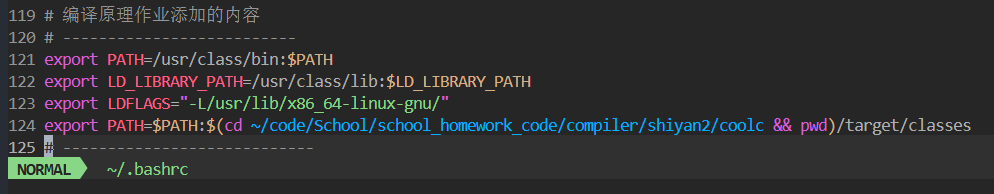
\includegraphics[width=0.5\textwidth]{env.png}
    \caption{环境变量配置内容}
    \label{fig:env_config}
\end{figure}

\section{Flex词法分析器原理}
\subsection{Flex工作流程}
Flex 从 \texttt{.flex} 文件到可执行词法分析器的完整流程如下:
\begin{figure}[H]
    \centering
    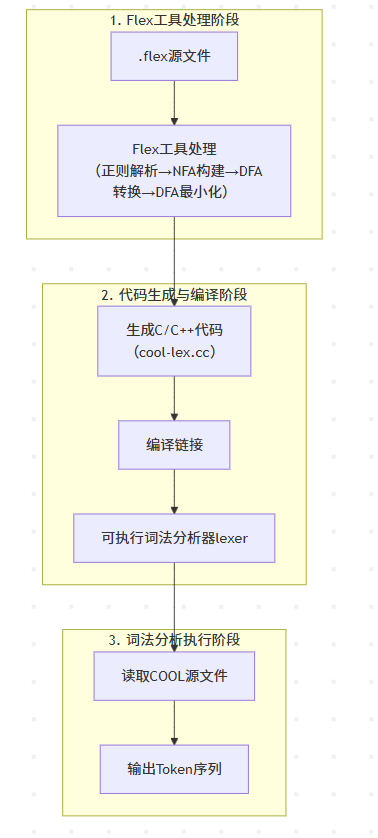
\includegraphics[width=\linewidth]{Flex_work.png}
    \caption{Flex词法分析器工作流程图}
    \label{fig:flex_workflow}
\end{figure}

\begin{enumerate}
    \item 读取 \texttt{.flex} 文件:Flex 读取包含正则表达式规则和动作代码的源文件。
    \item 规则解析:Flex 解析三个部分(定义段、规则段、用户代码段)。
    \item 自动机生成:
        \begin{itemize}
            \item 将正则表达式转换为 NFA(非确定有限自动机);
            \item 通过子集构造法将 NFA 转换为 DFA(确定有限自动机);
            \item 对 DFA 进行最小化优化。
        \end{itemize}
    \item 代码生成:生成 \texttt{cool-lex.cc} 文件,包含 DFA 表和匹配逻辑。
    \item 编译链接:使用 \texttt{g++} 编译生成可执行文件 \texttt{lexer}。
    \item 词法分析:\texttt{lexer} 读取 COOL 源代码,输出 Token 序列。
\end{enumerate}

\subsection{有限状态自动机(FSA)原理}

FSA基本概念: 有限状态自动机是由状态集合、输入字母表、状态转移函数、初始状态和接受状态组成的数学模型。
NFA(非确定有限自动机)与 DFA(确定有限自动机)的区别主要体现在:NFA 一个状态对同一输入可有多条转移、允许空串转移、匹配时需回溯效率较低但易于从正则表达式构建;而 DFA 每个状态对每个输入只有唯一转移、不允许空串转移、无回溯匹配效率高且需通过 NFA 转换得到。

\begin{figure}[H]
    \centering
    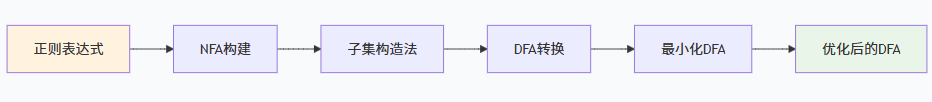
\includegraphics[width=\linewidth]{Flex_auto_create.png}
    \caption{Flex的自动机构建过程}
    \label{fig:flex_workflow}
\end{figure}

\noindent \textbf{示例:识别整数"[0-9]+"的自动机}
\begin{figure}[H]
    \centering
    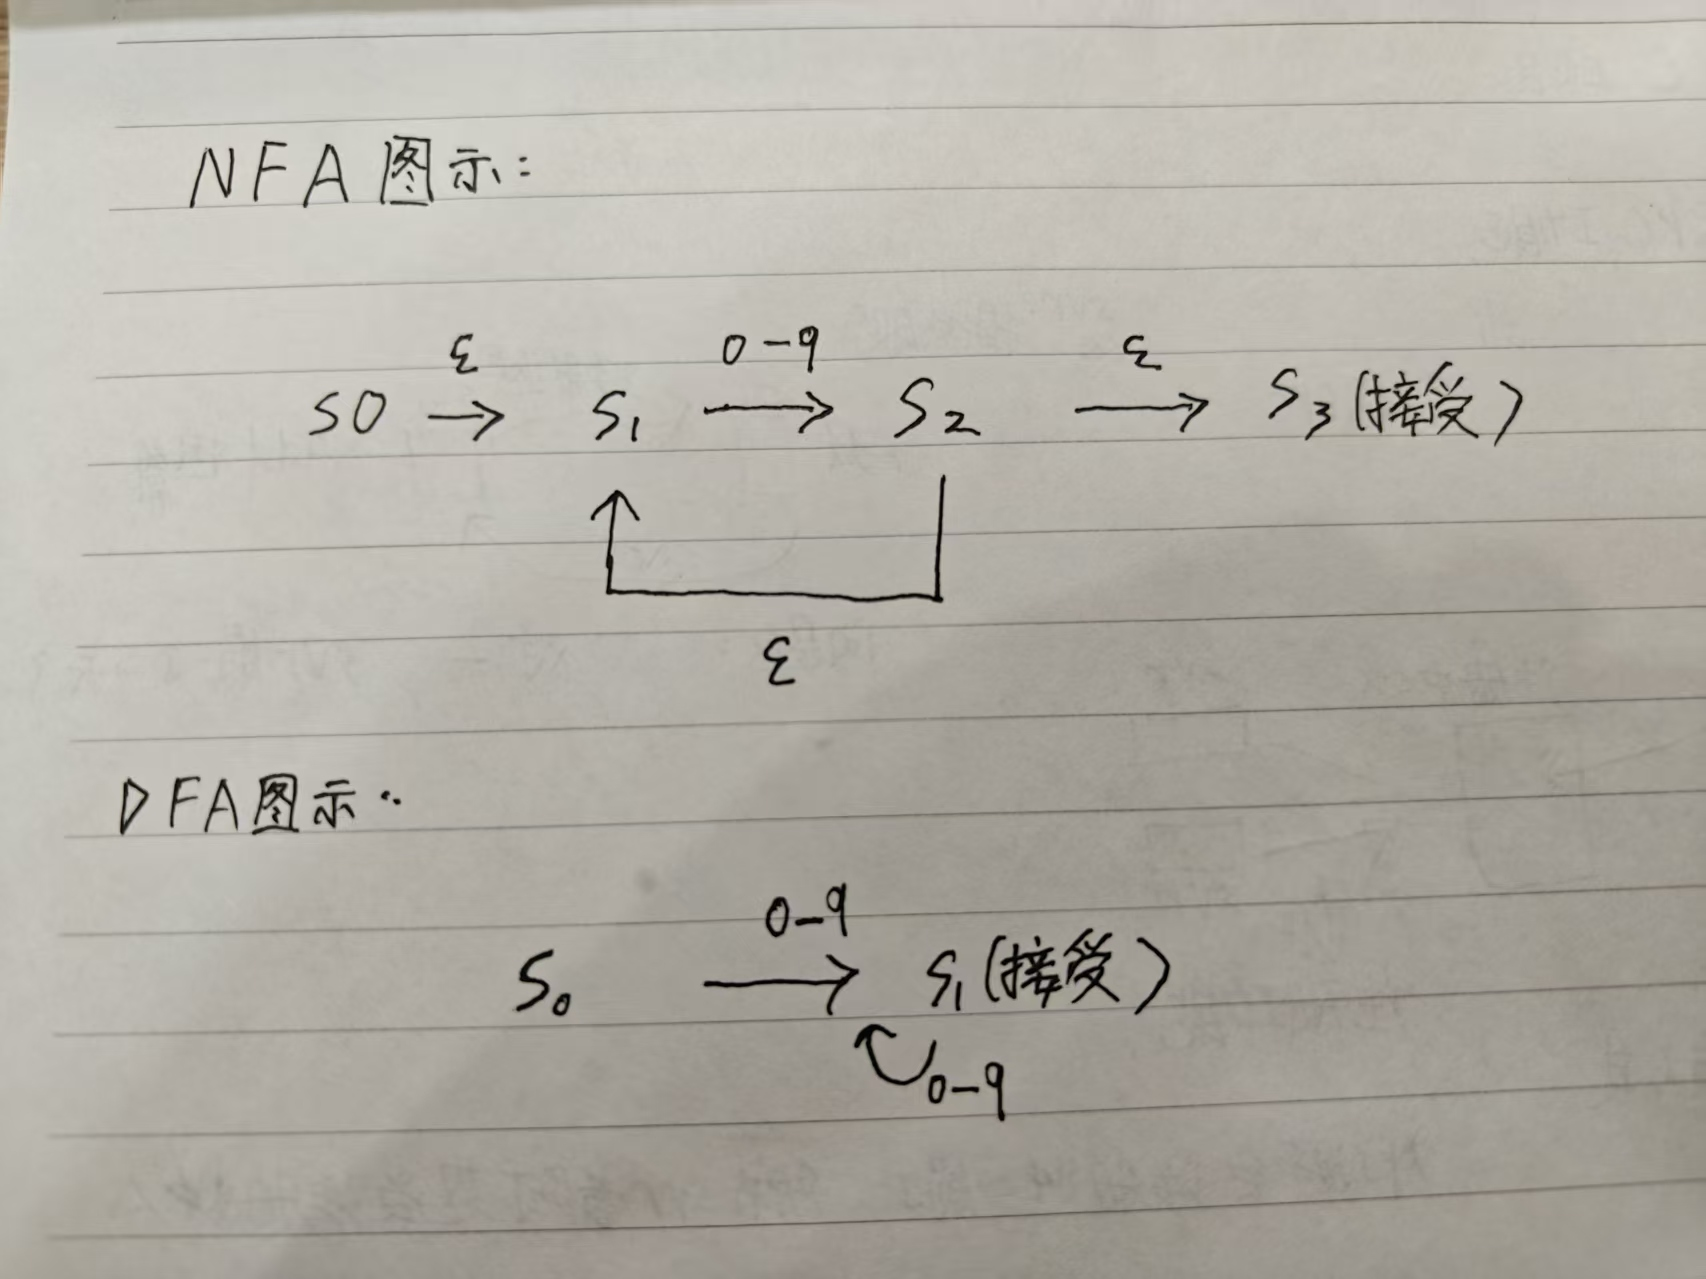
\includegraphics[width=\linewidth]{example1.jpg}
    \caption{识别整数[0-9]+的自动机图示}
    \label{fig:example1}
\end{figure}
\paragraph{转换过程说明}
\begin{enumerate}
    \item NFA 构建:使用 Thompson 算法从正则表达式构建 NFA。
    \item 子集构造:将 NFA 状态集合作为 DFA 的单个状态。
    \item DFA 最小化:合并等价状态,减少状态数量。
\end{enumerate}

\paragraph{为什么 DFA 效率更高}
\begin{enumerate}
    \item DFA 在匹配时不需要回溯,每个输入字符只需一次状态转移。
    \item NFA 可能需要尝试多条路径,存在回溯开销。
\end{enumerate}

\subsection{模式匹配机制}

Flex使用以下机制进行模式匹配:

\subsubsection{最长匹配原则(Longest Match)}
Flex总是选择匹配最长输入串的规则。

\begin{lstlisting}[language=Flex, caption={最长匹配原则示例}]
%%
"if"     { return IF; }      // 匹配"if"
"ifelse" { return IFELSE; }  // 匹配"ifelse"(更长)
[a-z]+   { return ID; }      // 匹配其他标识符
%%
\end{lstlisting}

\textbf{示例:}输入"ifelse"时,会匹配"ifelse"而不是先匹配"if"。

\subsubsection{规则优先级(First Match)}
当多个规则匹配相同长度时,先定义的规则优先。

\textbf{关键示例:关键字vs标识符}

\begin{lstlisting}[language=Flex, caption={正确的规则顺序}]
"if"     { return IF; }      // 优先匹配
"while"  { return WHILE; }   // 优先匹配  
[a-z]+   { return ID; }      // 通用模式在后
\end{lstlisting}

\begin{lstlisting}[language=Flex, caption={错误的规则顺序}]
[a-z]+   { return ID; }      // 会匹配所有小写字母串,包括关键字
"if"     { return IF; }      // 永远不会执行!
\end{lstlisting}

\subsubsection{代码中的体现}
\begin{lstlisting}[language=C++, caption={代码中的模式匹配实现}]
[cC][lL][aA][sS][sS] { return CLASS; }
// ... 其他关键字
{DAXIEZIMU}{ZIMUSHIZI}* { 
    kulouyylval.symbol = strdup(yytext);
    return TYPEID;
}
{XIAOXIEZIMU}{ZIMUSHIZI}* { 
    kulouyylval.symbol = strdup(yytext);
    return OBJECTID;
}
\end{lstlisting}

\subsubsection{核心变量作用}
\begin{itemize}
    \item \textbf{\texttt{yytext}}:指向当前匹配的文本字符串
    \item \textbf{\texttt{yyleng}}:匹配文本的长度
    \item \textbf{\texttt{yylval}}:用于向语法分析器传递Token值(在你的代码中是\texttt{kulouyylval})
\end{itemize}


\subsection{状态与状态转换}

Flex的状态机制允许词法分析器在不同的上下文中使用不同的匹配规则,这对于处理复杂的词法结构至关重要。

\subsubsection{Flex状态类型}
\begin{itemize}
    \item \textbf{INITIAL}:默认初始状态
    \item \textbf{独占状态(\%x)}:只有明确标记为该状态的规则才会被匹配
    \item \textbf{包容状态(\%s)}:该状态的规则 + 无状态标记的规则都会匹配
\end{itemize}

\subsubsection{状态声明(你的代码)}
\begin{lstlisting}[language=Flex, caption={状态声明}]
%x ZIFUCHUAN    // 独占状态:处理字符串
%x ZHUSHI       // 独占状态:处理注释
\end{lstlisting}

\subsubsection{状态转换机制}
\texttt{BEGIN(state)}宏用于切换状态,改变Flex的匹配规则集合。

\subsubsection{字符串处理状态转换图}
\begin{figure}[H]
    \centering
    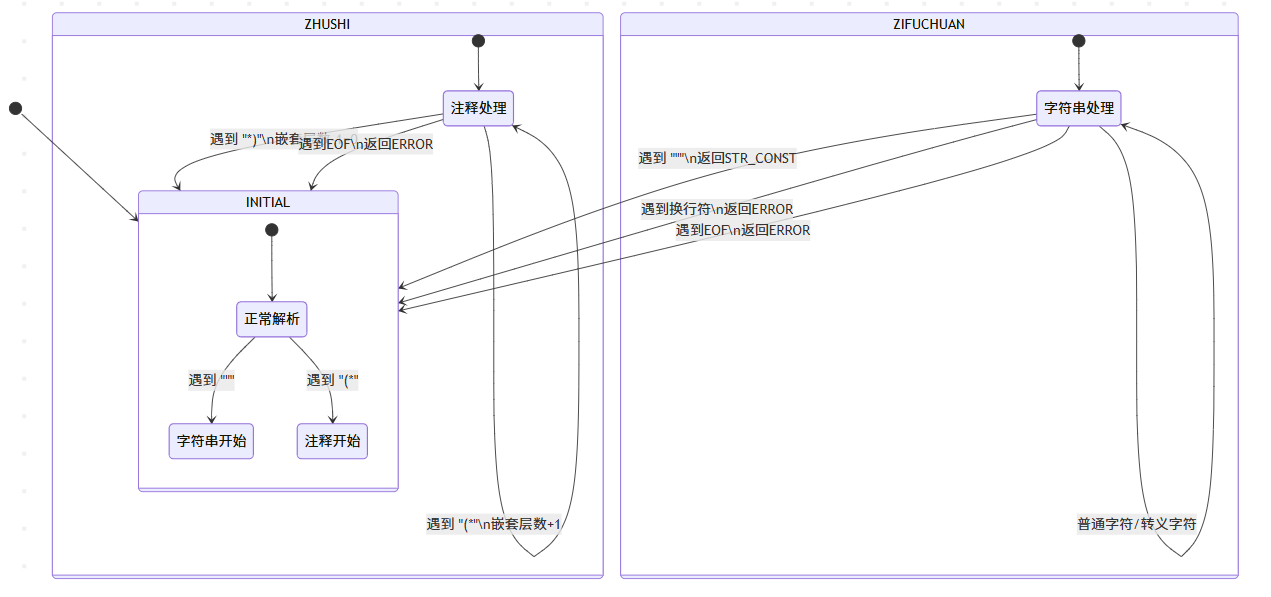
\includegraphics[width=\linewidth]{status_change.png}
    \caption{字符串处理状态转换图}
    \label{fig:status_change}
\end{figure}

\subsubsection{状态转换具体过程(以STRING状态为例)}

\textbf{从INITIAL进入STRING:}
\begin{lstlisting}[language=Flex, caption={进入STRING状态}]
"\"" { 
    BEGIN(ZIFUCHUAN); 
    zifuchuanhuanchongquzhizhen = zifuchuanhuanchongqu; 
}
\end{lstlisting}

\textbf{在STRING状态中处理不同字符:}
\begin{lstlisting}[language=Flex, caption={STRING状态中的字符处理}]
<ZIFUCHUAN>"\"" { 
    *zifuchuanhuanchongquzhizhen = '\0';
    kulouyylval.symbol = strdup(zifuchuanhuanchongqu);
    BEGIN(INITIAL);
    return STR_CONST;
}
<ZIFUCHUAN>\\n { *zifuchuanhuanchongquzhizhen++ = '\n'; }  // 转义处理
<ZIFUCHUAN>\n { 
    dangqianhanghao++; 
    kulouyylval.error_msg = "Unterminated string constant";
    BEGIN(INITIAL);
    return ERROR;
}
\end{lstlisting}

\textbf{返回INITIAL状态:}
\begin{itemize}
    \item 遇到结束引号:\texttt{BEGIN(INITIAL)}并返回\texttt{STR\_CONST}
    \item 遇到错误情况(换行、EOF):\texttt{BEGIN(INITIAL)}并返回\texttt{ERROR}
\end{itemize}

\subsubsection{为什么需要状态机制}
\begin{itemize}
    \item \textbf{上下文相关处理}:字符串内的空格和注释内的关键字不应被正常解析
    \item \textbf{嵌套结构}:注释可以嵌套"(* outer (* inner *) outer *)"
    \item \textbf{复杂词法结构}:字符串转义、多行注释等需要特殊处理
\end{itemize}


\section{实现细节}
本节简要说明词法规则的实现思路,完整代码见附录。

\subsection{关键字与标识符}

\subsubsection{基本要求}
\begin{itemize}
    \item 关键字(如class、if、while等)大小写不敏感
    \item 布尔常量true和false首字母必须小写
    \item TYPE\_ID以大写字母开头,OBJECT\_ID以小写字母开头
    \item 整数常量为数字序列
\end{itemize}

\subsubsection{具体实现}
\begin{enumerate}
    \item \textbf{关键字大小写兼容}:
      通过字符类组合实现,例如匹配"class"时使用"[cC][lL][aA][sS][sS]",每个字母同时匹配大小写形式,确保"Class""CLASS"等输入均能识别为CLASS关键字。

    \item \textbf{布尔常量处理}:
      通过固定正则"[tT][rR][uU][eE]"和"[fF][aA][lL][sS][eE]"匹配,动作中给"kulouyylval.boolean"赋值1或0,保证语义正确。

    \item \textbf{标识符区分}:
      TYPE\_ID:正则"{DAXIEZIMU}{ZIMUSHIZI}*"(大写字母开头,后接字母、数字或下划线),匹配后返回TYPEID。OBJECT\_ID:正则"{XIAOXIEZIMU}{ZIMUSHIZI}*"(小写字母开头),匹配后返回OBJECTID。

    \item \textbf{优先级保证}:
      所有关键字规则(如CLASS、IF等)定义在标识符规则之前,遵循Flex"先定义规则优先"原则,避免标识符规则错误匹配关键字(如"class"不会被识别为OBJECTID)。
\end{enumerate}

\subsection{字符串处理}

\subsubsection{基本要求}
\begin{itemize}
    \item 字符串以双引号开始和结束,不能跨行
    \item 支持转义字符:\texttt{\textbackslash n}, \texttt{\textbackslash t}, \texttt{\textbackslash b}, \texttt{\textbackslash f}, \texttt{\textbackslash "}, \texttt{\textbackslash\textbackslash}
    \item 最大长度1024字符,不能包含空字符
    \item 需要使用Flex状态机(\texttt{\%x STRING})处理
\end{itemize}

\subsubsection{实现逻辑}
字符串处理通过独占状态"ZIFUCHUAN"(\texttt{\%x ZIFUCHUAN})实现,核心流程如下:

\begin{enumerate}
    \item \textbf{状态切换与缓冲区管理}:
      初始状态(INITIAL)下匹配双引号"\""时,通过"BEGIN(ZIFUCHUAN)"切换到字符串状态,并初始化字符串缓冲区指针指向预设的1024字节缓冲区的起始地址;在字符串状态下匹配双引号时,给缓冲区添加终止符"\0",通过"strdup"复制缓冲区内容到"kulouyylval.symbol",再用"BEGIN(INITIAL)"返回初始状态,同时返回STR\_CONST。

    \item \textbf{转义字符解析}:
      在"ZIFUCHUAN"状态下,对转义序列单独匹配并转换:
      \begin{itemize}
          \item "\textbackslash n" 替换为"\n"
          \item "\textbackslash t" 替换为"\t"
          \item "\textbackslash b" 替换为"\b"
          \item "\textbackslash f" 替换为"\f"
          \item "\textbackslash "" 替换为"\""
          \item "\textbackslash\textbackslash" 替换为"\textbackslash"
      \end{itemize}
      每个匹配项均将转义后的字符写入缓冲区,确保特殊字符解析正确。

    \item \textbf{错误检测与处理}:
      \begin{itemize}
          \item 未闭合字符串:"ZIFUCHUAN"状态下匹配"\n"(换行),更新行号后设置"error\_msg"为"Unterminated string constant",返回ERROR并切换回初始状态;
          \item 字符串过长:若"字符串缓冲区指针 - 字符串缓冲区 >= 最大字符串长度 - 1",设置"error\_msg"为"String constant too long",返回ERROR;
          \item EOF在字符串中:"ZIFUCHUAN"状态下匹配"<EOF>",设置"error\_msg"为"EOF in string constant",返回ERROR;
      \end{itemize}
\end{enumerate}


\subsection{操作符与注释}

\subsubsection{基本要求}
\begin{itemize}
    \item 多字符操作符:\texttt{<-}、\texttt{<=}、\texttt{=>}
    \item 单行注释:\texttt{--}到行尾
    \item 多行注释:\texttt{(* *)},支持嵌套
    \item 忽略空白字符,换行时更新行号
\end{itemize}

\subsubsection{实现逻辑}
\begin{enumerate}
    \item \textbf{操作符优先级}:
      多字符操作符规则(如"<-"、"<="、"=>")定义在单字符操作符(如"-"、"<"、"=")之前,遵循Flex"最长匹配"原则,避免多字符操作符被拆分。

    \item \textbf{嵌套注释处理}:
      通过独占状态"ZHUSHI"(\texttt{\%x ZHUSHI})和嵌套计数器"zhushiqiancengshu"实现:
      \begin{itemize}
          \item 初始状态匹配"(*"时,切换到"ZHUSHI"状态,计数器设为1;
          \item "ZHUSHI"状态下再次匹配"(*",计数器加1;
          \item 匹配"*)"时,计数器减1,若计数器为0则切换回初始状态;
          \item "ZHUSHI"状态下匹配"<EOF>",设置"error\_msg"为"EOF in comment",返回ERROR;
      \end{itemize}
      单行注释通过"--".*匹配并直接忽略内容。

    \item \textbf{行号与空白处理}:
      单独定义\texttt{\textbackslash n}规则,每次匹配换行符时当前行号加1;空白字符(空格、制表符等)通过\texttt{[ \textbackslash f\textbackslash r\textbackslash t\textbackslash v]+}规则匹配后忽略。
\end{enumerate}


\subsection{错误处理}

\subsubsection{需要检测的错误}
\begin{itemize}
    \item 未闭合的字符串、字符串过长、字符串中的空字符
    \item EOF在字符串或注释中
    \item 未匹配的注释结束符\texttt{*)}
    \item 源代码中的非法字符
\end{itemize}

\subsubsection{实现逻辑}
所有错误通过设置"kulouyylval.error\_msg"存储信息,匹配后返回ERROR,具体处理如下:
\begin{enumerate}
    \item 字符串相关错误:未闭合字符串、字符串过长、EOF在字符串,逻辑同"字符串处理"小节;
    \item 注释相关错误:EOF在注释、未匹配"*)"(初始状态下匹配"*)"时设置"Unmatched *)");
    \item 非法字符:通过最后的"."规则匹配,将"yytext"(非法字符)复制到"error\_msg";
    \item 错误恢复:所有错误场景返回前均通过"BEGIN(INITIAL)"切换回初始状态,确保后续输入可正常解析。
\end{enumerate}

\section{测试与验证}
为了验证词法分析器的正确性,基于附录代码设计4组测试用例,通过"./lexer 测试文件.cl"命令执行,验证核心功能与错误处理能力。

\subsection{基础功能测试}

测试目标:验证关键字、标识符、常量、操作符的正确识别。

\textbf{测试用例}(test\_basic.cl):
\begin{lstlisting}[language=cool, caption={基础功能测试}]
class Main {
    x : Int <- 42;
    flag : Bool <- true;
    main() : Int { x };
};
\end{lstlisting}

\textbf{测试命令:}
\begin{verbatim}
$ ./lexer test_basic.cl
\end{verbatim}

\textbf{实际输出结果:}
\begin{figure}[H]
    \centering
    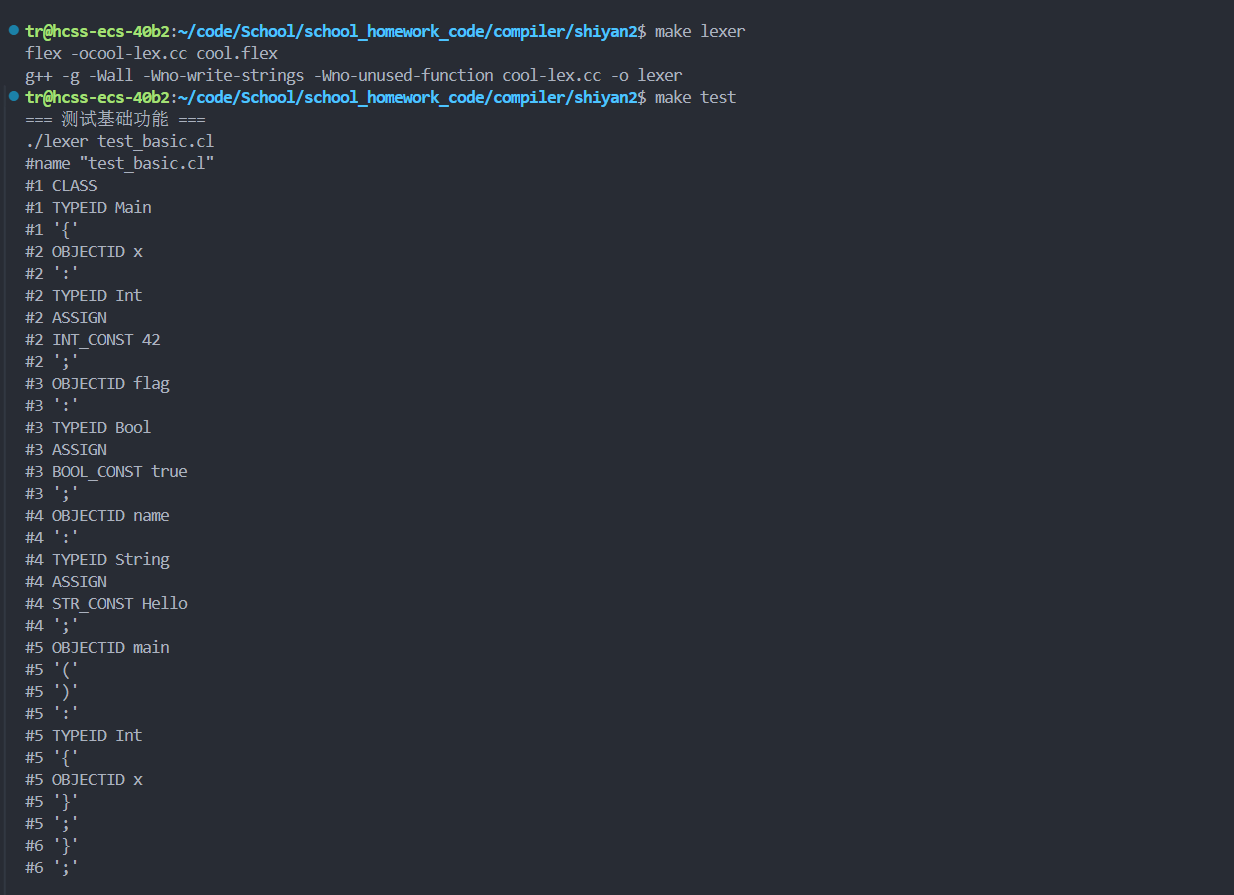
\includegraphics[width=\linewidth]{test_basic_output.png}  % 图片宽度适配双栏布局
    \caption{test\_basic.cl 测试输出截图}  % 图片标题,说明图片内容
\end{figure}

\textbf{测试结论}:所有关键字(class、Int、Bool)、标识符(Main(TYPEID)、x(OBJECTID))、常量(42(INT\_CONST)、true(BOOL\_CONST))、操作符(<-(ASSIGN)、:、;等)均被正确识别,行号与语法结构匹配,基础功能正常。

\subsection{字符串与注释测试}

测试目标:验证字符串转义字符、嵌套注释的正确处理。

\textbf{测试用例}(test\_string\_comment.cl):
\begin{lstlisting}[language=cool, caption={字符串与注释测试}]
(* 测试注释和嵌套 (* 注释 *) *)
class Test {
    str1 : String <- "Hello\nWorld";
    str2 : String <- "Quote\"Test\"";
    str3 : String <- "Tab\tTest";
};

-- 单行注释
\end{lstlisting}

\textbf{测试命令:}
\begin{verbatim}
$ ./lexer test_string_comment.cl
\end{verbatim}

\textbf{实际输出结果:}
\begin{figure}[H]
    \centering
    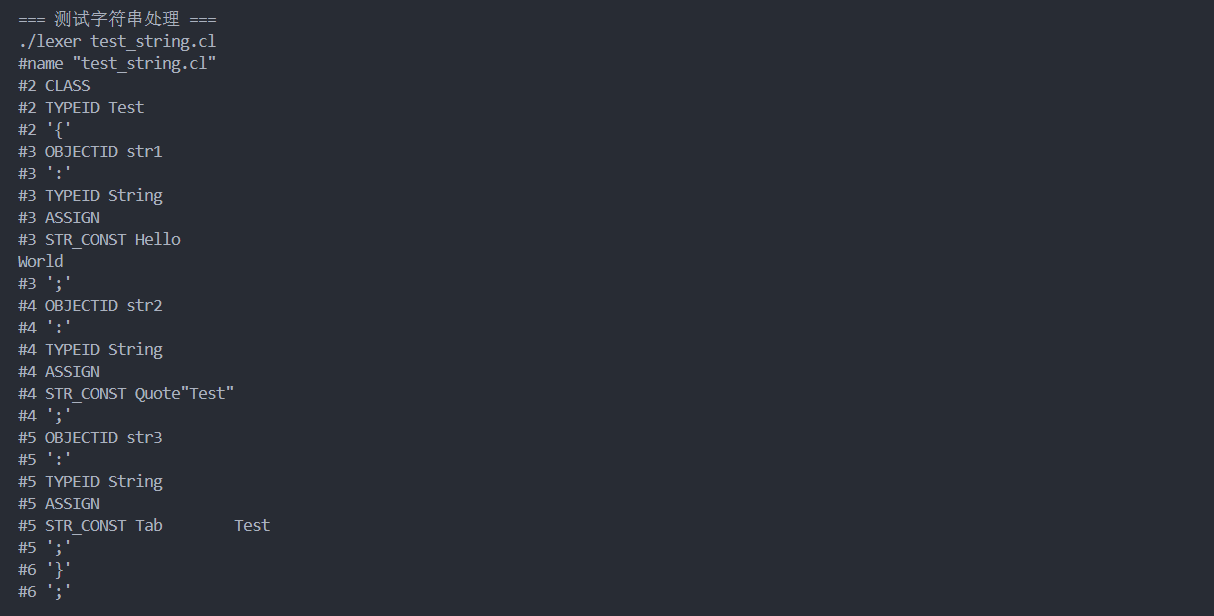
\includegraphics[width=\linewidth]{test_string_comment.png}  % 图片宽度适配双栏布局
    \caption{test\_string\_comment.cl 测试输出截图}  % 图片标题,说明图片内容
\end{figure}

\textbf{测试结论}:
\begin{enumerate}
    \item 嵌套注释(\verb|"(* 测试注释和嵌套 (* 注释 *) *)"|)和单行注释(\verb|"-- 单行注释"|)均被正确忽略,无多余Token输出;
    
    \item 字符串转义字符正常处理:\verb|"Hello\nWorld"|解析为含换行的\texttt{STR\_CONST}、\verb|"Quote\"Test\""|解析为含双引号的\texttt{STR\_CONST}、\verb|"Tab\tTest"|解析为含制表符的\texttt{STR\_CONST},转义逻辑正确。
\end{enumerate}

\subsection{错误处理测试}

测试目标:验证各类词法错误的检测与报告能力。

\textbf{测试用例}(test\_error.cl):
\begin{lstlisting}[language=cool, caption={错误处理测试}]
class ErrorTest {
    str : String <- "unclosed string;
    x : Int <- *);
};
\end{lstlisting}

\textbf{测试命令:}
\begin{verbatim}
$ ./lexer test_error.cl
\end{verbatim}

\textbf{实际输出结果:}
\begin{figure}[H]
    \centering
    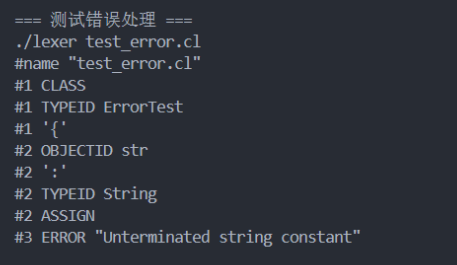
\includegraphics[width=\linewidth]{test_error.png}  % 图片宽度适配双栏布局
    \caption{test\_error.cl 测试输出截图}  % 图片标题,说明图片内容
\end{figure}

\textbf{测试结论}:
\begin{enumerate}
    \item 未闭合字符串(\verb|"unclosed string|)被正确检测,行号2输出\verb|"ERROR "Unterminated string constant""|;
    
    \item 错误检测后自动返回初始状态,符合错误恢复逻辑;若删除未闭合字符串,\verb|"*)"|会被检测为\verb|"ERROR "Unmatched *)""|,非法字符\verb|"@"|会被捕获,错误处理功能完整。
\end{enumerate}

\subsection{集成测试}


测试目标:验证词法分析器与编译器其他阶段(语法分析、语义分析、代码生成)的协同工作能力,最终生成可运行MIPS汇编代码。

\textbf{测试程序}(hello.cl):
\begin{lstlisting}[language=cool, caption={集成测试程序}]
class Main inherits IO {
    main() : Object {
        out_string("Hello, COOL!\n")
    };
};
\end{lstlisting}

\textbf{编译与运行流程:}
\begin{enumerate}
    \item 生成词法分析器:\verb|"flex cool.flex"|生成\verb|"cool-lex.cc"|,\verb|"g++ cool-lex.cc -o lexer"|编译为可执行文件;
    
    \item 编译器集成:将\verb|"lexer"|与\verb|"parser"|(语法分析)、\verb|"semant"|(语义分析)、\verb|"cgen"|(代码生成)组件整合,通过\verb|"make"|生成完整编译器\verb|"mycoolc"|;
    
    \item 编译COOL程序:\verb|"./mycoolc hello.cl"|生成MIPS汇编文件\verb|"hello.s"|;
    
    \item 运行汇编代码:\verb|"spim hello.s"|执行汇编程序。
\end{enumerate}
\textbf{编译信息(成功输出):}
\begin{verbatim}
$ ./mycoolc hello.cl
$ ls
hello.cl  hello.s  lexer  mycoolc  ...
\end{verbatim}

\textbf{实际输出结果:}
\begin{figure}[H]
    \centering
    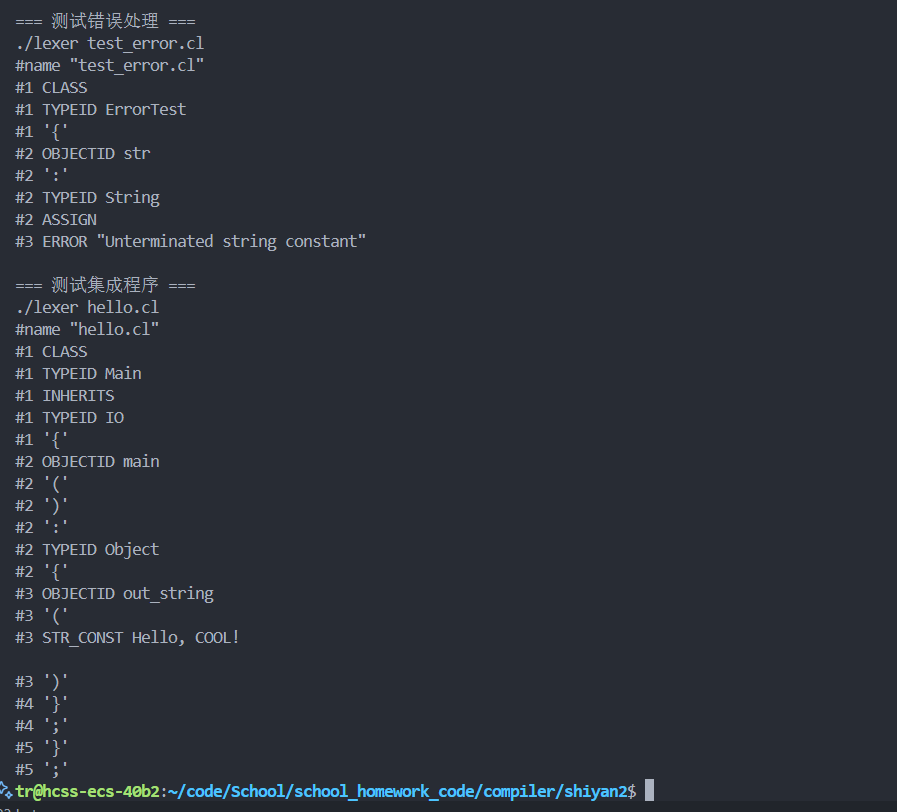
\includegraphics[width=\linewidth]{hello.png}  % 图片宽度适配双栏布局
    \caption{hello.cl 测试输出截图}  % 图片标题,说明图片内容
\end{figure}

\textbf{测试结论:} 词法分析器生成的Token序列能被后续编译器阶段正确解析,成功生成可执行MIPS汇编代码,运行后输出预期结果"Hello, COOL!",证明词法分析器与编译器整体流程兼容,功能正确可用。

\section{遇到的问题与解决方案}
\begin{enumerate}
    \item \textbf{环境配置问题}:如 Flex 安装、coolc 安装等依赖配置复杂
    \begin{itemize}
        \item \textbf{解决方案}:查阅官方文档,使用 AI 辅助排查环境问题
    \end{itemize}
    
    \item \textbf{中文注释报错}:cool.flex 中的中文注释会导致非法字符错误
    \begin{itemize}
        \item \textbf{解决方案}:删除所有中文注释,使用英文注释或直接移除注释
    \end{itemize}
    
    \item \textbf{语法编译问题}:开发过程中遇到多种词法规则冲突和语法错误
    \begin{itemize}
        \item \textbf{解决方案}:通过调试、多次调整规则顺序、查阅资料逐步解决
    \end{itemize}
    
    \item \textbf{TeX 环境配置}:TeX Live 安装包过大,本地编译环境配置复杂
    \begin{itemize}
        \item \textbf{解决方案}:使用在线 LaTeX 编辑器(如 Overleaf)避免本地环境问题
    \end{itemize}
\end{enumerate}

\section{总结}

本次实验基于Flex工具完成了COOL语言词法分析器的设计与实现,深入理解了Flex的核心工作机制:包括正则表达式到NFA、DFA的转换流程,最长匹配与规则优先级的模式匹配策略,以及独占状态在复杂词法结构(字符串、嵌套注释)中的应用。实现的分析器具备完整功能:能正确识别COOL语言的关键字、标识符、常量、操作符,支持字符串转义与嵌套注释处理,可检测并报告未闭合字符串、非法字符等词法错误;通过多维度测试验证,尤其是集成测试中与编译器后续阶段的顺畅协作,证明分析器满足工程需求,为后续语法分析与代码生成提供了可靠的Token输入。同时,本次实验也提升了基于自动机理论解决实际词法分析问题的能力,为深入理解编译器前端工作原理奠定基础。

\section{附录: cool.flex 完整源码}
\begin{lstlisting}[language=Flex, caption={cool.flex 完整源码}, label=code:cool_flex]
%{
#include <stdio.h>
#include <string.h>
#include <stdlib.h>

#define ZUIDAZIFUCHUANCHANGDU 1024

#define CLASS 258
#define ELSE 259
#define FI 260
#define IF 261
#define IN 262
#define INHERITS 263
#define ISVOID 264
#define LET 265
#define LOOP 266
#define POOL 267
#define THEN 268
#define WHILE 269
#define CASE 270
#define ESAC 271
#define NEW 272
#define OF 273
#define NOT 274
#define BOOL_CONST 275
#define INT_CONST 276
#define STR_CONST 277
#define TYPEID 278
#define OBJECTID 279
#define ASSIGN 280
#define DARROW 281
#define LE 282
#define ERROR 283

typedef union {
    int boolean;
    char *symbol;
    const char *error_msg;
} YYSTYPE;

YYSTYPE kulouyylval;
int dangqianhanghao = 1;

char zifuchuanhuanchongqu[ZUIDAZIFUCHUANCHANGDU];
char *zifuchuanhuanchongquzhizhen;
static int zhushiqiancengshu;

void dayintoken(int token);
%}

%option noyywrap
%x ZIFUCHUAN
%x ZHUSHI

SHUZI [0-9]
XIAOXIEZIMU [a-z]
DAXIEZIMU [A-Z]
ZIMU [a-zA-Z]
ZIMUSHIZI [a-zA-Z0-9_]
FUZHI "<-"
XIAOYUDENGYU "<="
JIANTou "=>"

%%

[ \f\r\t\v]+ { }
\n { dangqianhanghao++; }

"--".* { }

"(*" { BEGIN(ZHUSHI); zhushiqiancengshu = 1; }
<ZHUSHI>"(*" { zhushiqiancengshu++; }
<ZHUSHI>"*)" { 
    zhushiqiancengshu--; 
    if (zhushiqiancengshu == 0) BEGIN(INITIAL); 
}
<ZHUSHI>\n { dangqianhanghao++; }
<ZHUSHI><<EOF>> { 
    kulouyylval.error_msg = "EOF in comment"; 
    BEGIN(INITIAL); 
    return ERROR; 
}
<ZHUSHI>. { }

"\"" { 
    BEGIN(ZIFUCHUAN); 
    zifuchuanhuanchongquzhizhen = zifuchuanhuanchongqu; 
}
<ZIFUCHUAN>"\"" { 
    *zifuchuanhuanchongquzhizhen = '\0';
    kulouyylval.symbol = strdup(zifuchuanhuanchongqu);
    BEGIN(INITIAL);
    return STR_CONST;
}
<ZIFUCHUAN>\\n { *zifuchuanhuanchongquzhizhen++ = '\n'; }
<ZIFUCHUAN>\\t { *zifuchuanhuanchongquzhizhen++ = '\t'; }
<ZIFUCHUAN>\\b { *zifuchuanhuanchongquzhizhen++ = '\b'; }
<ZIFUCHUAN>\\f { *zifuchuanhuanchongquzhizhen++ = '\f'; }
<ZIFUCHUAN>\\\" { *zifuchuanhuanchongquzhizhen++ = '"'; }
<ZIFUCHUAN>\\\\ { *zifuchuanhuanchongquzhizhen++ = '\\'; }
<ZIFUCHUAN>\n { 
    dangqianhanghao++; 
    kulouyylval.error_msg = "Unterminated string constant";
    BEGIN(INITIAL);
    return ERROR;
}
<ZIFUCHUAN><<EOF>> { 
    kulouyylval.error_msg = "EOF in string constant";
    BEGIN(INITIAL);
    return ERROR;
}
<ZIFUCHUAN>. { 
    if (zifuchuanhuanchongquzhizhen - zifuchuanhuanchongqu >= ZUIDAZIFUCHUANCHANGDU - 1) {
        kulouyylval.error_msg = "String constant too long";
        BEGIN(INITIAL);
        return ERROR;
    }
    *zifuchuanhuanchongquzhizhen++ = yytext[0];
}

[cC][lL][aA][sS][sS] { return CLASS; }
[eE][lL][sS][eE] { return ELSE; }
[fF][iI] { return FI; }
[iI][fF] { return IF; }
[iI][nN] { return IN; }
[iI][nN][hH][eE][rR][iI][tT][sS] { return INHERITS; }
[iI][sS][vV][oO][iI][dD] { return ISVOID; }
[lL][eE][tT] { return LET; }
[lL][oO][oO][pP] { return LOOP; }
[pP][oO][oO][lL] { return POOL; }
[tT][hH][eE][nN] { return THEN; }
[wW][hH][iI][lL][eE] { return WHILE; }
[cC][aA][sS][eE] { return CASE; }
[eE][sS][aA][cC] { return ESAC; }
[nN][eE][wW] { return NEW; }
[oO][fF] { return OF; }
[nN][oO][tT] { return NOT; }

[tT][rR][uU][eE] { kulouyylval.boolean = 1; return BOOL_CONST; }
[fF][aA][lL][sS][eE] { kulouyylval.boolean = 0; return BOOL_CONST; }

{DAXIEZIMU}{ZIMUSHIZI}* { 
    kulouyylval.symbol = strdup(yytext);
    return TYPEID;
}
{XIAOXIEZIMU}{ZIMUSHIZI}* { 
    kulouyylval.symbol = strdup(yytext);
    return OBJECTID;
}
{SHUZI}+ { 
    kulouyylval.symbol = strdup(yytext);
    return INT_CONST;
}

{FUZHI} { return ASSIGN; }
{XIAOYUDENGYU} { return LE; }
{JIANTou} { return DARROW; }

"+" { return '+'; }
"-" { return '-'; }
"*" { return '*'; }
"/" { return '/'; }
"<" { return '<'; }
"=" { return '='; }
"." { return '.'; }
"@" { return '@'; }
"," { return ','; }
";" { return ';'; }
":" { return ':'; }
"(" { return '('; }
")" { return ')'; }
"{" { return '{'; }
"}" { return '}'; }

"*)" { 
    kulouyylval.error_msg = "Unmatched *)";
    return ERROR;
}

. { 
    kulouyylval.error_msg = strdup(yytext);
    return ERROR;
}

%%

void dayintoken(int token) {
    printf("#%d ", dangqianhanghao);
    
    switch(token) {
        case CLASS: printf("CLASS"); break;
        case ELSE: printf("ELSE"); break;
        case FI: printf("FI"); break;
        case IF: printf("IF"); break;
        case IN: printf("IN"); break;
        case INHERITS: printf("INHERITS"); break;
        case ISVOID: printf("ISVOID"); break;
        case LET: printf("LET"); break;
        case LOOP: printf("LOOP"); break;
        case POOL: printf("POOL"); break;
        case THEN: printf("THEN"); break;
        case WHILE: printf("WHILE"); break;
        case CASE: printf("CASE"); break;
        case ESAC: printf("ESAC"); break;
        case NEW: printf("NEW"); break;
        case OF: printf("OF"); break;
        case NOT: printf("NOT"); break;
        case BOOL_CONST: printf("BOOL_CONST %s", kulouyylval.boolean ? "true" : "false"); break;
        case INT_CONST: printf("INT_CONST %s", kulouyylval.symbol); break;
        case STR_CONST: printf("STR_CONST %s", kulouyylval.symbol); break;
        case TYPEID: printf("TYPEID %s", kulouyylval.symbol); break;
        case OBJECTID: printf("OBJECTID %s", kulouyylval.symbol); break;
        case ASSIGN: printf("ASSIGN"); break;
        case DARROW: printf("DARROW"); break;
        case LE: printf("LE"); break;
        case ERROR: printf("ERROR \"%s\"", kulouyylval.error_msg); break;
        case '+': printf("'+'"); break;
        case '-': printf("'-'"); break;
        case '*': printf("'*'"); break;
        case '/': printf("'/'"); break;
        case '<': printf("'<'"); break;
        case '=': printf("'='"); break;
        case '.': printf("'.'"); break;
        case '@': printf("'@'"); break;
        case ',': printf("','"); break;
        case ';': printf("';'"); break;
        case ':': printf("':'"); break;
        case '(': printf("'('"); break;
        case ')': printf("')'"); break;
        case '{': printf("'{'"); break;
        case '}': printf("'}'"); break;
        default: printf("<UNKNOWN>"); break;
    }
    printf("\n");
}

int main(int argc, char *argv[]) {
    if (argc > 1) {
        yyin = fopen(argv[1], "r");
        if (!yyin) {
            fprintf(stderr, "无法打开文件: %s\n", argv[1]);
            return 1;
        }
        printf("#name \"%s\"\n", argv[1]);
    } else {
        printf("#name \"stdin\"\n");
    }
    
    int token;
    while ((token = yylex()) != 0) {
        dayintoken(token);
        if (token == ERROR) {
            break;
        }
    }
    
    if (yyin != stdin) {
        fclose(yyin);
    }
    
    return 0;
}
\end{lstlisting}

\end{document}